\documentclass[11pt]{article} 
\usepackage{amssymb, amsmath, amsthm}
\usepackage{tikz, graphicx, color, mathrsfs, rotating}
\usepackage{titlesec, lipsum}
\usepackage{fancyhdr, framed, chngcntr}

\usetikzlibrary{arrows,shapes,automata,backgrounds,decorations,petri,positioning,patterns}


\paperwidth = 8.5in
\paperheight = 11in
\textwidth = 6.5 in
\textheight = 9 in
\oddsidemargin = 0 in
\evensidemargin = 0 in
\topmargin = -.25 in
\headheight = 0.0 in
\headsep = .25 in
\footskip = .25in


\newtheorem*{repp@prob}{\repp@title}
\newcommand{\newreppprob}[2]{
\newenvironment{repp#1}[1]{
 \def\repp@title{#2 {##1}}
 \begin{repp@prob}}
 {\end{repp@prob}}}
\makeatother
\newreppprob{prob}{Problem}

\newtheorem*{repp@thm}{\repp@title}
\newcommand{\newreppthm}[2]{
\newenvironment{repp#1}[1]{
 \def\repp@title{#2 {##1}}
 \begin{repp@thm}}
 {\end{repp@thm}}}
\makeatother
\newreppthm{thm}{Theorem}


% -----------------------------------------------------------------------------
%             Macros for the course
% -----------------------------------------------------------------------------
\newcommand{\TS}{\mathcal{T}} % symbol for a topological space
\newcommand{\BS}{\mathcal{B}} % symbol for a basis
\newcommand{\R}{\mathbb{R}} % symbol for real numbers
\newcommand{\Z}{\mathbb{Z}} % symbol for integers
\newcommand{\Q}{\mathbb{Q}} % symbol for rational numbers
\newcommand{\PS}{\mathscr{P}} % symbol for power set
\newcommand{\E}{\mathbf{E}} % symbol for real numbers with Euclidean topology
\newcommand{\F}{\mathbf{F}^1} % symbol for real numbers with finite-complement topology
\renewcommand{\H}{\mathbf{H}^1} % symbol for real numbers with half-open topology
\renewcommand{\S}{\mathcal{S}} % basis topology
\newcommand{\B}{\mathbf{B}} % symbol for ball
\newcommand{\Sp}{\mathbf{S}} % symbol for sphere
\renewcommand{\int}{\operatorname{int}} % symbol for interior
\newcommand{\bnd}{\partial} % symbol for boundary
\newcommand{\homeo}{\approx} % symbol for homeomorphic


\begin{document} 


% -----------------------------------------------------------------------------
%             Start here
% -----------------------------------------------------------------------------

{\large
\noindent School of Computing %% replace "date" by the date on which the assignment was made
\hfill Chansu Park %% replace "Name" by your name

\vspace{.1in}

\noindent \today \hfill 20173245}

\vspace{.25in}

% -----------------------------------------------------------------------------
%             Erase or rearrange the options below, as necessary
% -----------------------------------------------------------------------------
\Large{
\begin{center}
\textbf{CS580}

Spring 2018, Homework \#3
\end{center}
}

\large

% -----------------------------------------------------------------------------
%             Template for typing up an Exercise
% -----------------------------------------------------------------------------
Here is the sample image of my work:
\begin{figure}[htb]
	\begin{center}
		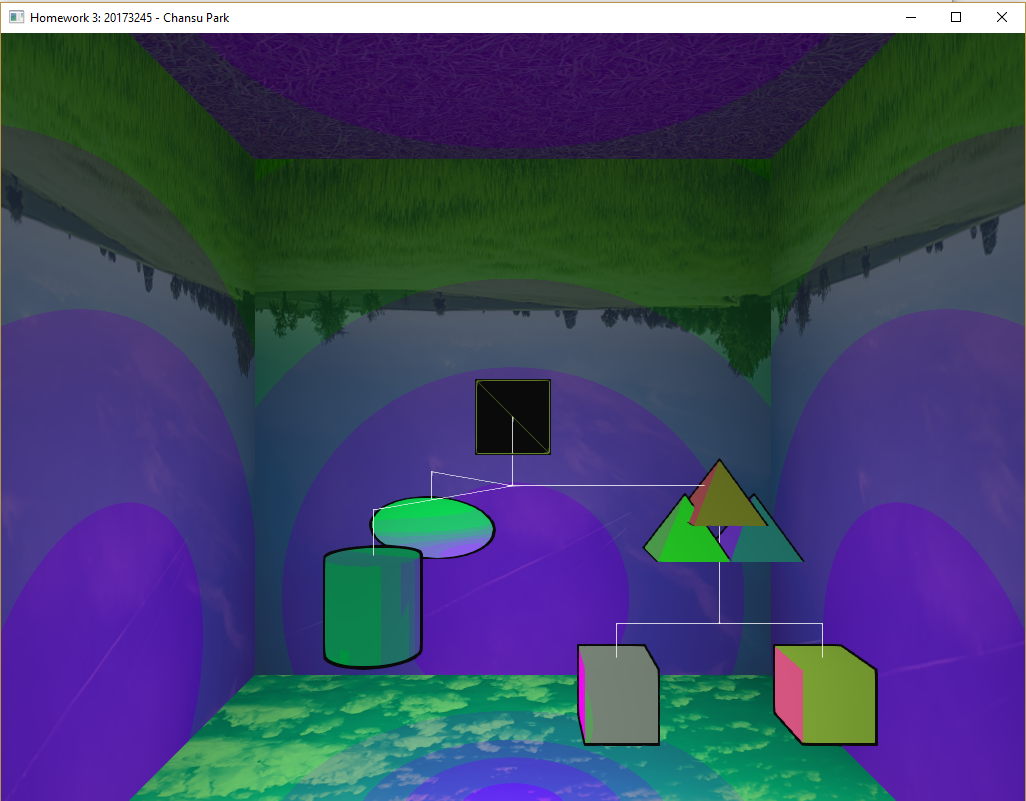
\includegraphics[width=0.8\linewidth]{gooch.png}
	\end{center}
	\caption{A sample picture with a point light with both gooch shading and toon shading. Outlines are seen in the scene.}
\end{figure}

\section{Scene Setting} \label{sec:1}
Actually, I didn't introduce new complex mesh object.

I also didn't visualize the position of the point light, but made it moving around $x$-axis. You can adjust the speed of the rotation of the point light using 7 and 8 on you keyboard.

\section{Non-Photorealistic Rendering} \label{sec:2}
\subsection{Rendering Style} \label{ssec:2.1}
I applied two types of shading methods: Gooch Shading and Toon Shading.
\begin{itemize}
	\item [Gooch:] Gooch shading is the method that computes the color using linear interpolation of `warm' color and `cool' color.
	To generate the warm color and cool color, it takes two base colors (call $c_{warm}$ and $c_{cool}$) and the diffuse reflectance (call $c_{point}$) of the point on the model.
	\[k_{warm} = c_{warm} + \alpha c_{point}; \qquad k_{cool} = c_{cool} + \beta c_{point}; \] \[0 \leq \alpha, \beta \leq 1, (0,0,0) \leq k_{warm}, k_{cool} \leq (1,1,1).\]
	The interpolating factor is computed using dot product of the light vector and the surface normal. The resulting color is following:
	\[I = \frac{1 + \vec{l} \cdot \vec{n}}{2} k_{cool} + \frac{1 - \vec{l} \cdot \vec{n}}{2} k_{warm}.\]
	I used different base colors for objects and walls: $k_{cool} = (0,0.7,0), k_{warm} = (0.6, 0, 0.6)$ for objects; $k_{cool} = (0, 0.5, 0), k_{warm} = (0.4, 0, 0.7)$ for walls.
	\item [Toon:]
	Then I discretized colors to enable Toon shading using the same interpolating factor used for Gooch shading.
	Note that, since the light is contained in the walls, I used different discretizing criteria for walls from objects.
	\begin{figure}[htb]
		\begin{center}
			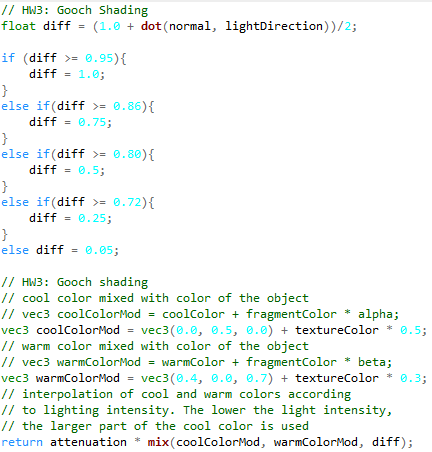
\includegraphics[width=0.6\linewidth]{goochtexture.png}
		\end{center}
		\caption{Gooch shading for textured objects (in this case, walls). Note that I finally inserted attenuation term.}
	\end{figure}
\end{itemize}
\subsection{Outlining} \label{ssec:2.2}
There are several outlining methods, but since I planned to use shadow map, geometry information was not needed. Thus I just used enlarged models and culled front faces.
\begin{figure}[htb]
	\begin{center}
		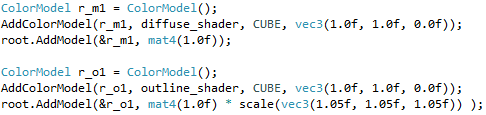
\includegraphics[width=0.7\linewidth]{scaledModel.png}
	\end{center}
	\caption{For each model, I attached scaled model at the same location. These models will have almost black colors.}
\end{figure}
\begin{figure}[htb]
	\begin{center}
		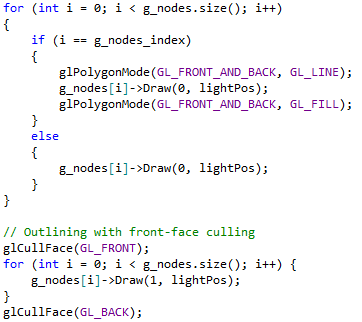
\includegraphics[width=0.5\linewidth]{judgeOutline.png}
	\end{center}
	\caption{Each nodes draws the actual model or the outline according to the first argument they receive.}
\end{figure}

\newpage
\section{Shadow} \label{sec:3}
I tried to implement shadow mapping, but I didn't finish that since it required depth cubemap which was quite complex to set.

\section{Directory hierarchy}
I worked on \texttt{Visual Studio 2015 Professional Win64}.

I attached the whole sources from the skeleton zip file since I edited several files.

You can see the images I used for textures in the \texttt{./Resources/images/}.

For the executable, the \texttt{Executable} folder contains the copy of the executable from \texttt{./build/Debug} with shaders from \texttt{./Skeleton}.

There is also a pdf file containing this document in the root. Hope you to see this program.

%\begin{proof}[Solution.]
%% write your solution here
%\end{proof}


% -----------------------------------------------------------------------------
%             Template for typing up a Theorem
% -----------------------------------------------------------------------------
%\begin{reppthm}{42} %% replace "42" by the relevant Theorem number
%% restate the Theorem here
%\end{reppthm}

%\begin{proof}
%% write your proof here
%\end{proof}


% -----------------------------------------------------------------------------
%             End here
% -----------------------------------------------------------------------------

\end{document}